% ===================================================================================================
\chapter{Results}
% ===================================================================================================

% ----------------------------------------------------------------------------------
\section{Vacancies}
% ----------------------------------------------------------------------------------
In Fig. \ref{Fig:1Vac_results} and \ref{Fig:2Vac_results} we can see the number of T and H atoms bound to the mono- and divacancies as a function of time and at different temperatures. 
For comparison, the results of the monoisotopic, 'vacuum annealing', simulations are also shown. 
We can see that at all three temperatures, T-removal from the monovacancy occurs at a higher rate when isotope exchange is used, compared to the monoisotopic cases.
For the divacancies (Fig. \ref{Fig:2Vac_results}), the T-removal using isotope exchange occurs nearly as fast as in the monovacancy case, despite starting with nearly twice the amount T. 
While the difference in both cases is more prominent at lower temperatures, it is noticeable also at 500 K, where removal through pure diffusion starts to play a significant role.
Despite us aiming mainly for qualitative results, a semi-quantitative comparison reveals the T-removal rate to be around 50 times higher when employing isotope exchange compared to monoisotopic simulations in monovacancies. 

\begin{figure}[!ht]
\begin{subfigure}{.5\textwidth}
  \centering
  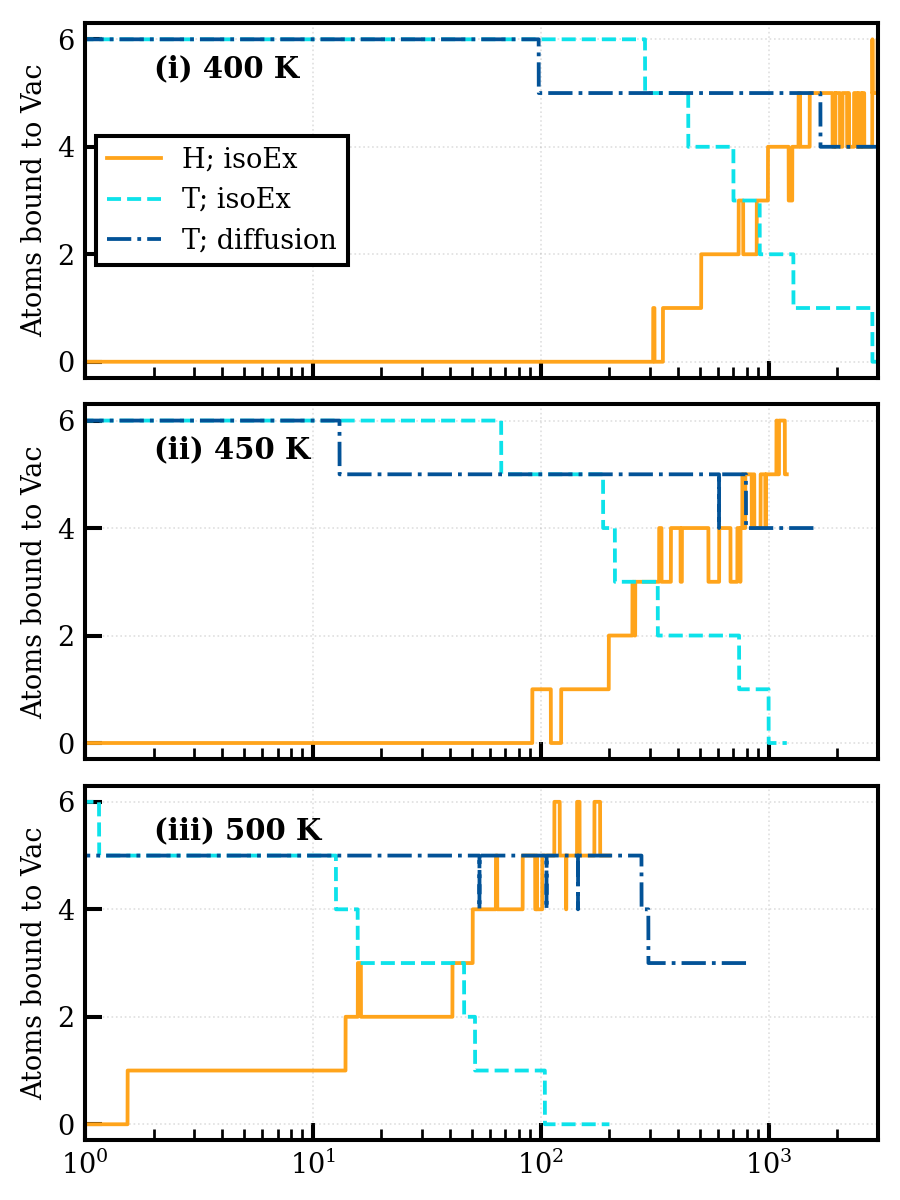
\includegraphics[width=0.99\textwidth]{1Vac_isoEx_HT_log.png}  
  \caption{Logarithmic time scale}
  %\label{fig:sub-first}
\end{subfigure}
\begin{subfigure}{.5\textwidth}
  \centering
  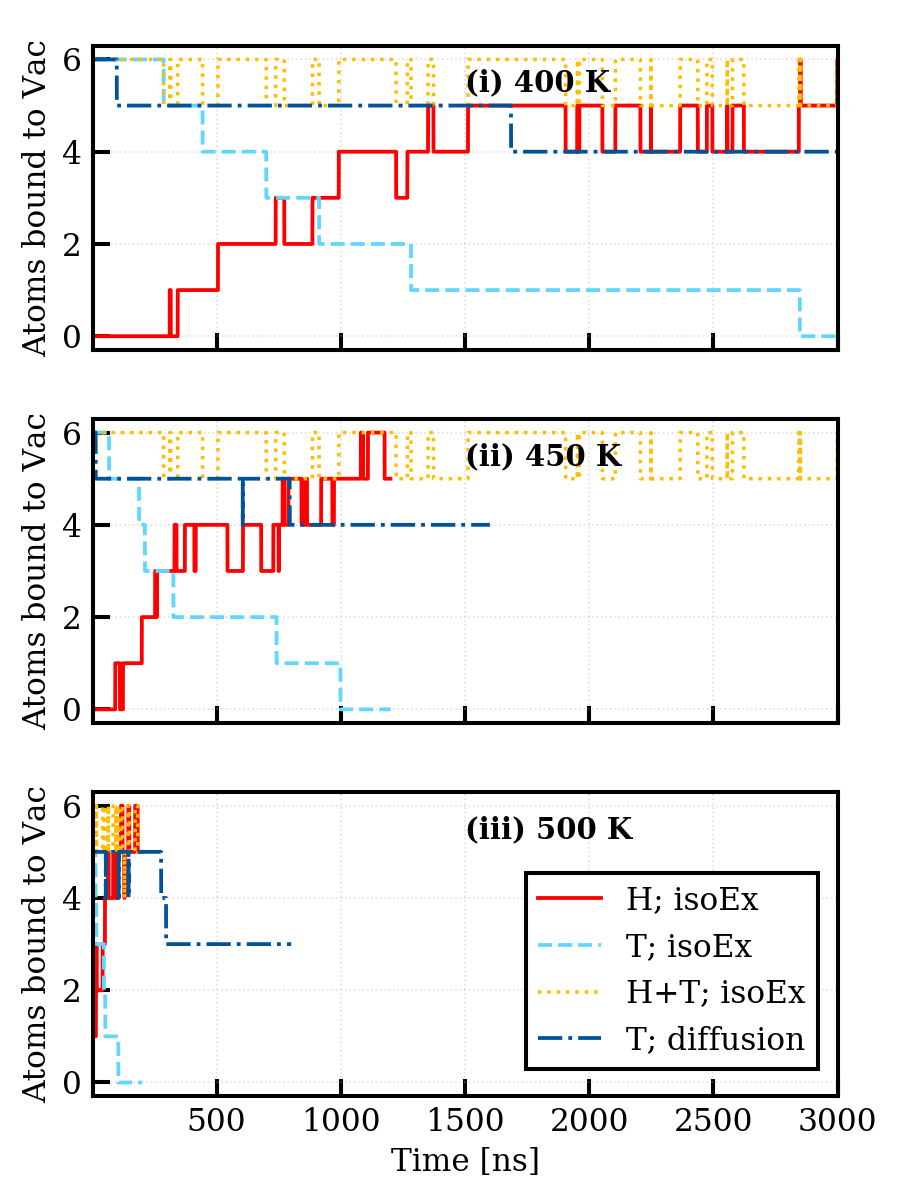
\includegraphics[width=0.99\textwidth]{1Vac_isoEx_HT.png}  
  \caption{Linear time scale}
  %\label{fig:sub-second}
\end{subfigure}
\caption{Number of H and T atoms bound to the monovacancy for isotope exchange and monoisotopic diffusion simulations. The number of trapped T in the monovacancy decreases much faster in the simulations with isotope exchange, compared to the monoisotopic cases.}
 \label{Fig:1Vac_results} 
\end{figure}


\begin{figure}[!ht]
\begin{subfigure}{.5\textwidth}
  \centering
 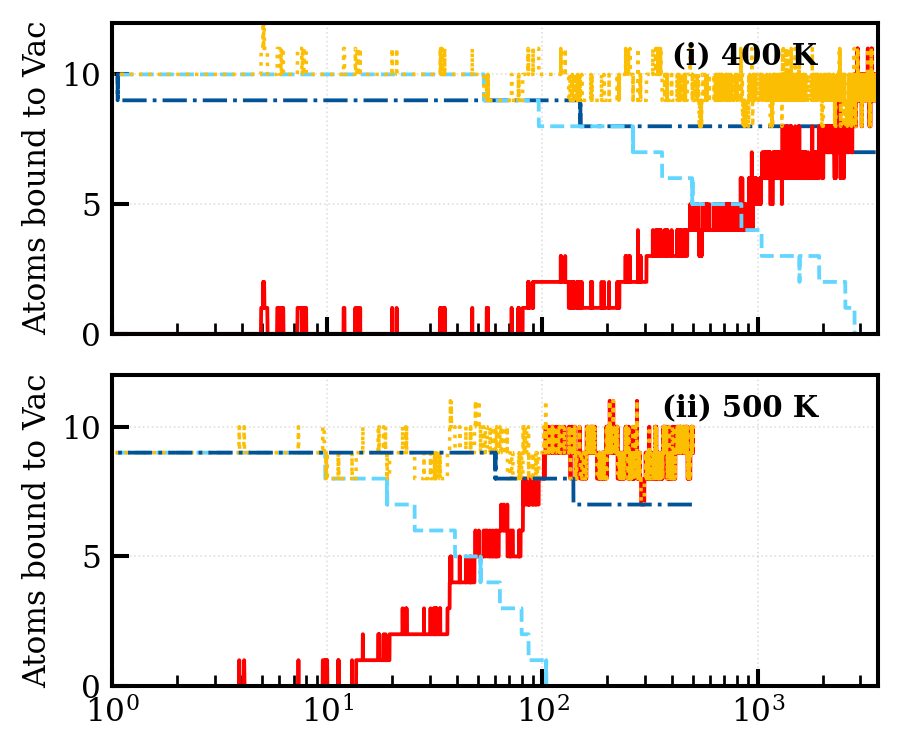
\includegraphics[width=0.99\textwidth]{2Vac_isoEx_HT_log.png}  
  \caption{Logarithmic time scale}
  %\label{fig:sub-first}
\end{subfigure}
\begin{subfigure}{.5\textwidth}
  \centering
  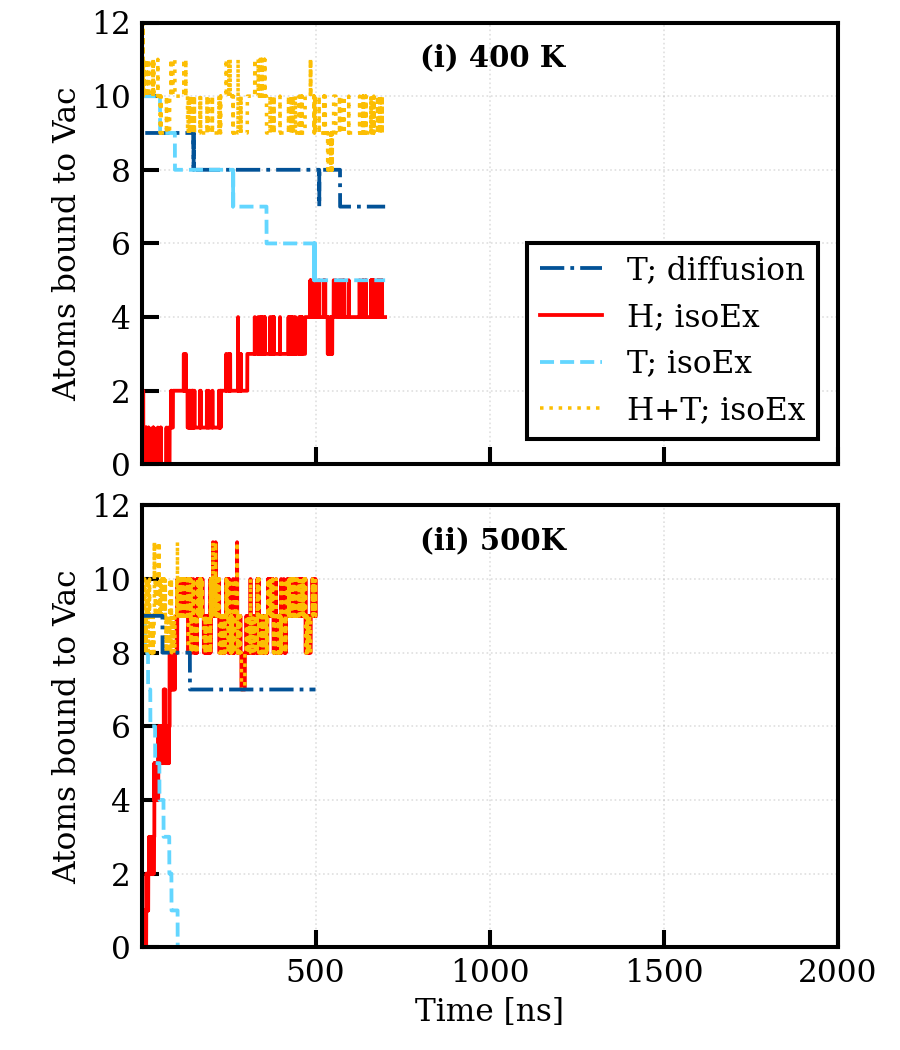
\includegraphics[width=0.99\textwidth]{2Vac_isoEx_HT.png}  
  \caption{Linear time scale}
  %\label{fig:sub-second}
\end{subfigure}
   \caption{Number of H and T atoms bound to the divacancy for isotope exchange and monoisotopic diffusion simulations. Despite the nearly doubled number of T, the removal with isotope exchange occurs at a similar rate than in the monovacancy simulations.}
   \label{Fig:2Vac_results} 
\end{figure}

The binding energies of the second to sixth H atoms bound monovacancy are systematically underestimated by the MD potential compared to the corresponding DFT values \cite{heinolaTungstenDFT}, Fig. \ref{Fig:Ebind1H_DFT}.
The DFT binding energy for the sixth H is around 0.3 eV, and above 0.8 eV for all the rest.
A consequence of this, assuming that the DFT binding energies indeed are accurate, is that in a real "vacuum annealing" experiment, annealing at below ca 500 K would only result in the detrapping of the sixth and loosest bound T.
The remaining five T would subsequently have very low probabilities of becoming detrapped.

In Fig. \ref{Fig:1Vac_results}, however, we see that about 2 to 3 T are detrapped from the vacancy in the monoisotopic simulation corresponding to 'vacuum annealing'.
This is a result of the too low MD binding energies plotted in Fig. \ref{Fig:Ebind1H_DFT}.
How would the present simulation results then change if the binding energies for the potential would be roughly the same as for DFT?
Firstly, there would probably be no less than five T bound to the monovacancy in the monoisotopic case, due to the relatively high binding energy of the fifth T (ca 0.8 eV).
Secondly, the effect on the isotope exchange results would be minor since, as seen in Fig. \ref{Fig:1Vac_results}, the combined amount of H and T in the monovacancy remains as five or six in all the simulations.
This means that only the sixth hydrogen atom is always detrapped and before any additional detrapping has occurred, a H (or T) atom has been trapped in its place.
Thus, an increase in the binding energies of the five first hydrogen atoms to the monovacancy should not affect the obtained results.

\begin{figure}[!ht]
	\center
	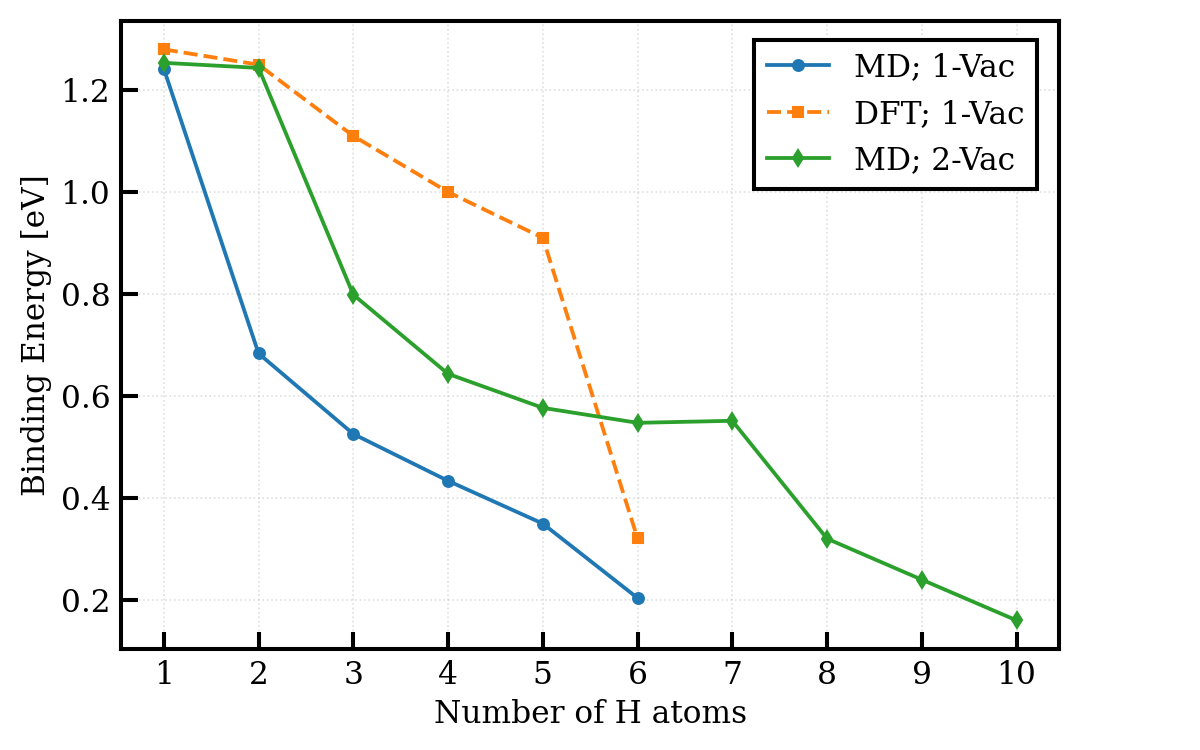
\includegraphics[width=0.55\linewidth]{Ebind.png}
	\caption{Comparision of the H-W binding energy in MD using the EAM1 potential by Bonny \textit{et. al} and DFT results by Heinola \textit{et. al. }\cite{heinolaTungstenDFT}}
	\label{Fig:Ebind1H_DFT}
\end{figure}

Plotting the potential energy of the individual T atoms as a function of time as in Fig. \ref{Fig:Epot}, we can see sharp fluctuations as the atoms move around inside the defect, transitioning in and out of binding energy states.
This seemingly irrelevant fact shows on an atomic level what has been hypothesised based on macroscopic observations to be the basis of the isotope exchange mechanism.
We can also see from both Fig. \ref{Fig:1Vac_results} and \ref{Fig:2Vac_results} that the combined number of T and H in the defects is kept roughly constant during the entirety of the simulations, with H atoms rapidly taking the place of detrapped T.

\begin{figure}[!ht]
	\center
	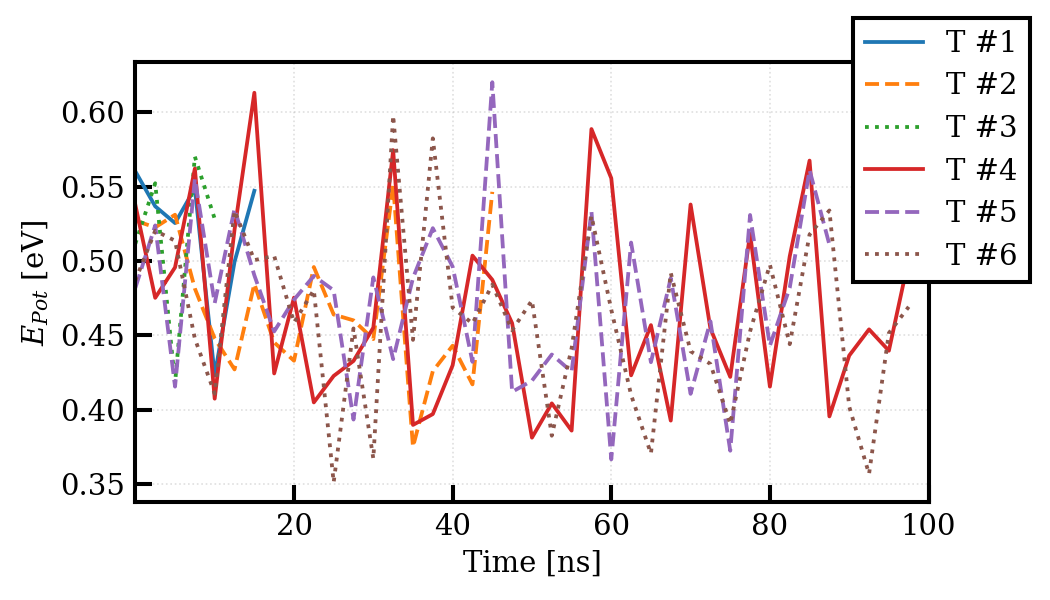
\includegraphics[width=0.55\linewidth]{epot.png}
	\caption{The potential energies of all individual T atoms in a 500 K simulation.\vspace*{6mm}}
	\label{Fig:Epot}
  %\label{fig:sub-second}
\end{figure}


% ----------------------------------------------------------------------------------
\section{Dislocations}
% ----------------------------------------------------------------------------------
The dislocation results are shown in Fig. \ref{Fig:disloc_results} and indicate an enhanced T-removal rate when utilising isotope exchange at 500 and 700 K. 
At 400 K, on the other hand, there is no significant difference between the two methods.

Comparing the T-removal rates at 700 K, we can conclude that total T-removal occurs around 10 times faster in the isotope exchange case compared to the monoisotopic case.
In comparison to the vacancy results in Fig. \ref{Fig:1Vac_results} and \ref{Fig:2Vac_results}, the overall T-removal rate for a dislocation appears to exceed that observed in the vacancies for both the isotope exchange and monoisotopic cases.
E.g. for the isotope exchange cases at 500 K we have normalised average T-removal rates, $\delta_{\text{T}}$, of 0.003 and 0.01 1/ns for a dislocation and a monovacancy, respectively.

Fig. \ref{Fig:disloc_results} additionally reveals that the total number of H and T bound to the defect increases slightly during the isotope exchange simulation, possibly due to insufficient saturation runs. 

\vspace{15mm} 

\begin{figure}[!ht]
\begin{subfigure}{.5\textwidth}
  \centering
 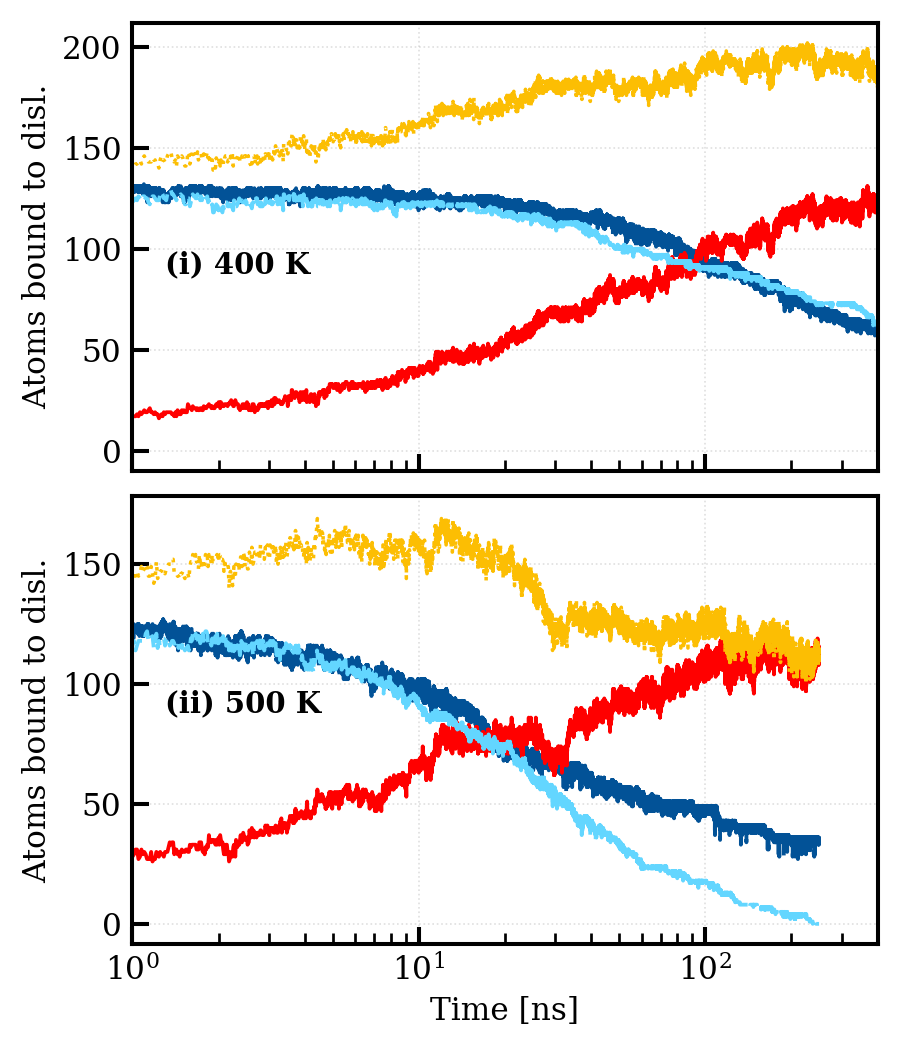
\includegraphics[width=0.99\textwidth]{disloc_isoEx_HT_log.png}  
  \caption{Logarithmic time scale}
  %\label{fig:sub-first}
\end{subfigure}
\begin{subfigure}{.5\textwidth}
  \centering
  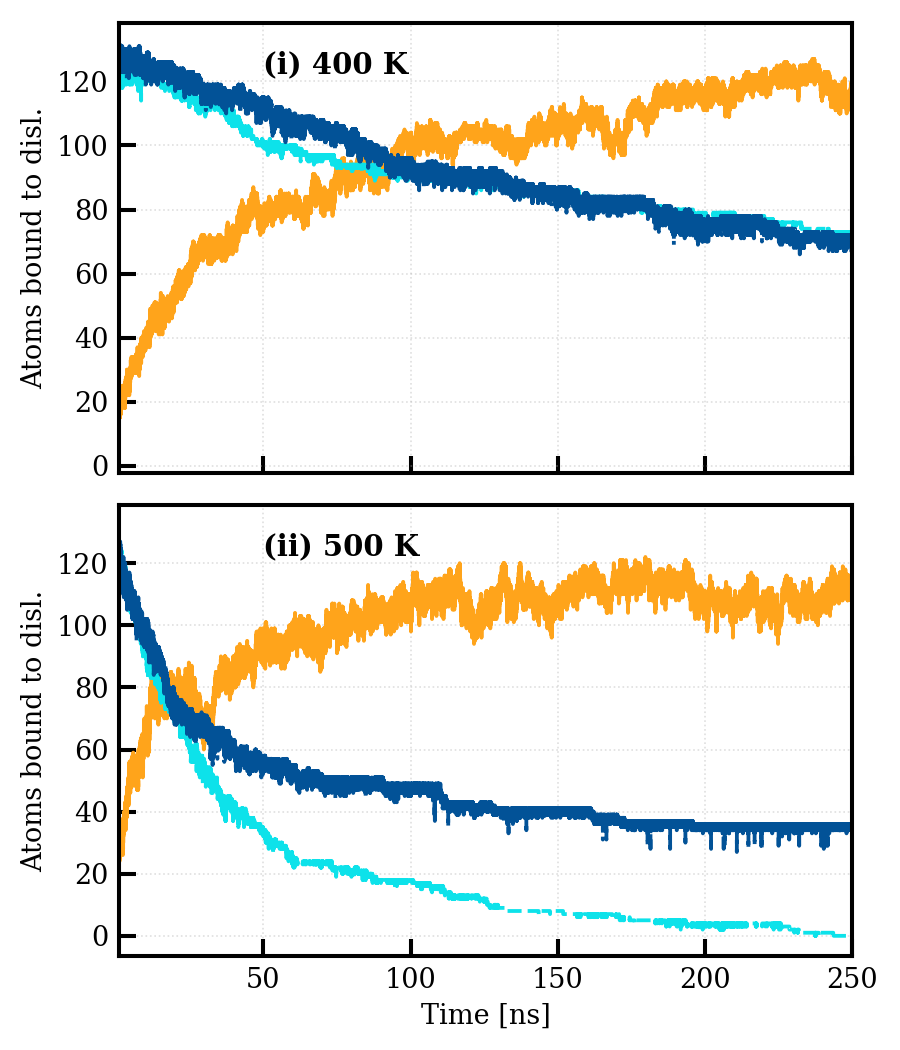
\includegraphics[width=0.99\textwidth]{disloc_isoEx_HT.png}  
  \caption{Linear time scale}
  %\label{fig:sub-second}
\end{subfigure}
   \caption{Number of H and T atoms bound to the dislocation for isotope exchange and monoisotopic diffusion simulations}
   \label{Fig:disloc_results} 
\end{figure}

\pagebreak

% ----------------------------------------------------------------------------------
\section{Grain boundaries}
% ----------------------------------------------------------------------------------
The grain boundary results are shown in Fig. \ref{Fig:GB_results}. 
Similarly to the dislocation case, a significant increase in the T-removal rate can be observed when isotope exchange is used at temperatures of at least 500 K.
The exact difference in removal rates was difficult to determine without excessive use of computing resources, but can be clearly seen from Fig. \ref{Fig:GB_results} to be several orders of magnitude higher for the isotope exchange simulations.

The normalised T-removal rate at 500 K was around $\delta_{\text{T}} = 0.0017$ 1/ns, i.e. around six times lower than the corresponding value for the monovacancy and half that of the dislocation.

\begin{figure}[!ht]
\begin{subfigure}{.5\textwidth}
  \centering
 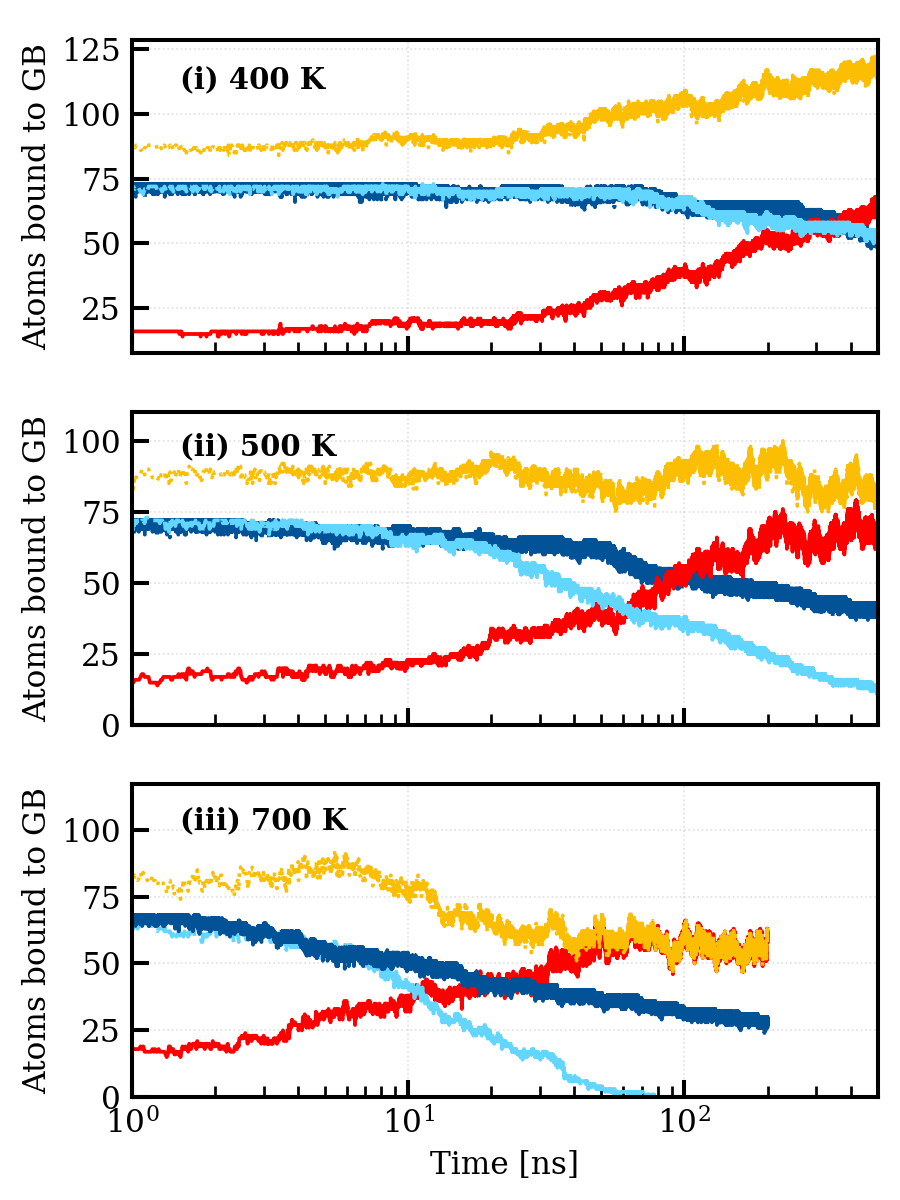
\includegraphics[width=0.99\textwidth]{GB_isoEx_HT_log.png}  
  \caption{Logarithmic time scale}
  %\label{fig:sub-first}
\end{subfigure}
\begin{subfigure}{.5\textwidth}
  \centering
  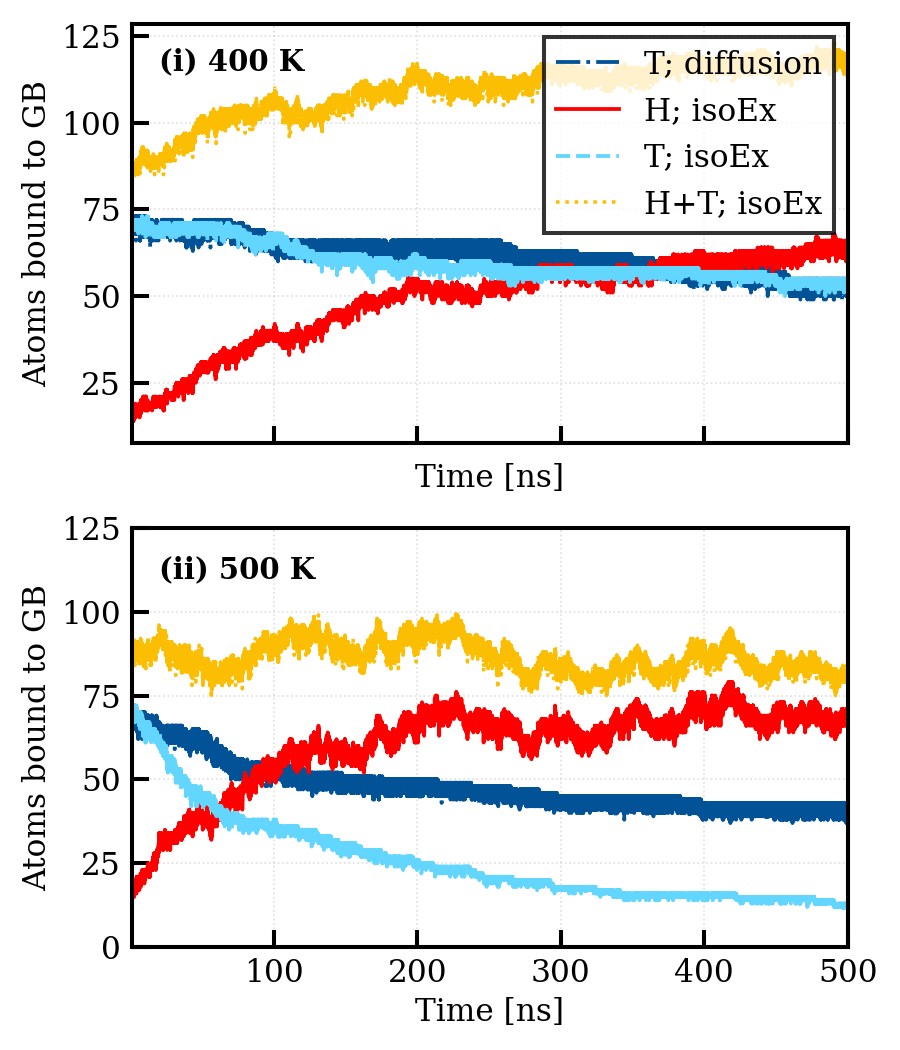
\includegraphics[width=0.99\textwidth]{GB_isoEx_HT.png}  
  \caption{Linear time scale}
  %\label{fig:sub-second}
\end{subfigure}
   \caption{Number of H and T atoms bound to the grain boundary for isotope exchange and monoisotopic diffusion simulations}
   \label{Fig:GB_results} 
\end{figure}

